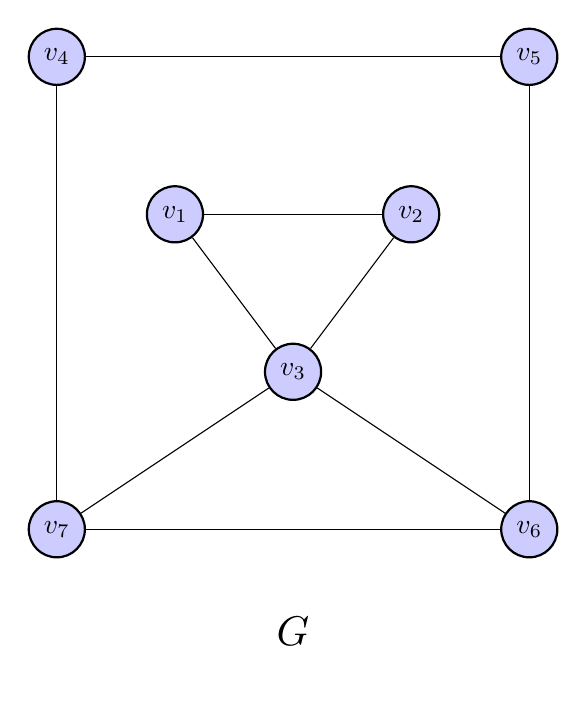
\begin{tikzpicture}[auto=left,every node/.style={circle,fill=blue!20,draw=black,thick}]
  % Cuadrado exterior (v4 y v5 en la parte superior; v7 y v6 en la parte inferior)
  \node (v4) at (-3, 3.5) {$v_4$};
  \node (v5) at (3, 3.5) {$v_5$};
  \node (v6) at (3, -2.5) {$v_6$};
  \node (v7) at (-3, -2.5) {$v_7$};

  % Triángulo interior (v1, v2, v3)
  \node (v1) at (-1.5, 1.5) {$v_1$};
  \node (v2) at (1.5, 1.5) {$v_2$};
  \node (v3) at (0, -0.5) {$v_3$};

  % Aristas del cuadrado exterior
  \foreach \from/\to in {v4/v5, v5/v6, v6/v7, v7/v4}
    \draw (\from) -- (\to);

  % Aristas del triángulo interior
  \foreach \from/\to in {v1/v2, v2/v3, v3/v1}
    \draw (\from) -- (\to);

  % Conexiones del vértice inferior v3 a las esquinas inferiores
  \draw (v3) -- (v7);
  \draw (v3) -- (v6);

  % Título
  \node[draw=none, fill=none, scale=1.5] at (0,-3.8) {$G$};
\end{tikzpicture}
